\documentclass[12pt,a4paper]{article}

% ── Packages ──────────────────────────────────────────────────────────────────
\usepackage[margin=2.5cm]{geometry}
\usepackage{amsmath,amssymb,amsthm}
\usepackage{listings}
\usepackage{xcolor}
\usepackage{hyperref}
\usepackage{booktabs}
\usepackage{graphicx}
\usepackage{tikz}
\usetikzlibrary{trees,shapes,arrows.meta,positioning}
\usepackage{fancyhdr}
\usepackage{titlesec}
\usepackage{enumitem}
\usepackage{tcolorbox}
\usepackage{fontenc}
\usepackage{inputenc}

% ── Colours ───────────────────────────────────────────────────────────────────
\definecolor{codeblue}{rgb}{0.13,0.29,0.53}
\definecolor{codegray}{rgb}{0.5,0.5,0.5}
\definecolor{codegreen}{rgb}{0.1,0.5,0.1}
\definecolor{backcolour}{rgb}{0.97,0.97,0.97}
\definecolor{aztecpurple}{RGB}{100,20,200}

% ── Listings style ────────────────────────────────────────────────────────────
\lstdefinestyle{tscode}{
  backgroundcolor=\color{backcolour},
  commentstyle=\color{codegreen},
  keywordstyle=\color{codeblue}\bfseries,
  numberstyle=\tiny\color{codegray},
  stringstyle=\color{orange},
  basicstyle=\ttfamily\small,
  breaklines=true,
  numbers=left,
  numbersep=8pt,
  tabsize=2,
  frame=single,
  rulecolor=\color{codegray},
  language=Java  % closest approximation for TypeScript highlighting
}

\lstdefinestyle{cppcode}{
  backgroundcolor=\color{backcolour},
  commentstyle=\color{codegreen},
  keywordstyle=\color{codeblue}\bfseries,
  numberstyle=\tiny\color{codegray},
  stringstyle=\color{orange},
  basicstyle=\ttfamily\small,
  breaklines=true,
  numbers=left,
  numbersep=8pt,
  tabsize=2,
  frame=single,
  rulecolor=\color{codegray},
  language=C++
}

% ── Header / footer ───────────────────────────────────────────────────────────
\pagestyle{fancy}
\fancyhf{}
\rhead{\textcolor{aztecpurple}{\textbf{Aztec Interview — Merkle Tree}}}
\lhead{\textit{Engineering Session Solution}}
\cfoot{\thepage}

% ── Title ─────────────────────────────────────────────────────────────────────
\title{
  \vspace{-1cm}
  {\color{aztecpurple}\rule{\linewidth}{2pt}}\\[0.4cm]
  \Huge\textbf{Merkle Tree Implementation}\\[0.3cm]
  \Large Aztec Engineering Interview — Full Solution\\[0.2cm]
  {\color{aztecpurple}\rule{\linewidth}{2pt}}
}
\author{Candidate Solution Document}
\date{March 2026}

% ── Theorem environments ──────────────────────────────────────────────────────
\newtheorem{definition}{Definition}
\newtheorem{theorem}{Theorem}
\newtheorem{property}{Property}
\newtheorem{algorithm}{Algorithm}

% ─────────────────────────────────────────────────────────────────────────────
\begin{document}
\maketitle
\tableofcontents
\newpage

% =============================================================================
\section{Problem Overview}
% =============================================================================

The challenge asks you to implement a \textbf{sparse binary Merkle tree} of
configurable depth, backed by a persistent key--value store.  Two identical
specifications are provided:

\begin{itemize}[leftmargin=1.5cm]
  \item \texttt{eng-sessions/merkle-tree/} — TypeScript, using LevelUp/memdown.
  \item \texttt{eng-sessions/merkle-tree-cpp/} — C++20, using a mock
        \texttt{unordered\_map} database.
\end{itemize}

Both require the \emph{same three operations}:

\begin{center}
\begin{tabular}{lll}
\toprule
\textbf{Method} & \textbf{TypeScript} & \textbf{C++} \\
\midrule
Constructor initialisation & \texttt{constructor(...)} & \texttt{MerkleTree(...)} \\
Membership proof & \texttt{getHashPath(index)} & \texttt{get\_hash\_path(index)} \\
Leaf update & \texttt{updateElement(index, value)} & \texttt{update\_element(index, value)} \\
\bottomrule
\end{tabular}
\end{center}

% =============================================================================
\section{Mathematical Background}
% =============================================================================

\subsection{Binary Merkle Trees}

\begin{definition}[Binary Merkle Tree]
A \emph{binary Merkle tree} of depth $d$ is a complete binary tree with
$2^d$ leaves.  Let $H : \{0,1\}^* \to \{0,1\}^{256}$ be a collision-resistant
hash function (here SHA-256).
\begin{itemize}
  \item \textbf{Leaf nodes} (level 0): given raw data $v_i$ of 64 bytes,
        $\ell_i = H(v_i)$.
  \item \textbf{Internal nodes} (levels $1 \ldots d$): for a node at position
        $(k, p)$ (level $k$, index $p$),
        \[
          n_{k,p} = H\!\bigl(n_{k-1,\,2p} \;\|\; n_{k-1,\,2p+1}\bigr).
        \]
  \item The \textbf{root} is $n_{d,0}$.
\end{itemize}
\end{definition}

\subsection{Tree Geometry}

With depth $d = 32$, the tree has $2^{32} \approx 4.3 \times 10^9$ leaf slots.
Leaves are addressed $0, 1, \ldots, 2^{32}-1$.  Given leaf index $i$:
\begin{itemize}
  \item Position at level $k$: $\; p_k(i) = \lfloor i / 2^k \rfloor = i \gg k$.
  \item Left-child position of a pair: $p_k(i) \mathbin{\&} \mathord{\sim}1$.
  \item Right-child position: $p_k(i) \mathbin{|} 1$.
  \item Sibling position: $p_k(i) \oplus 1$ (XOR with 1).
\end{itemize}

\subsection{Sparse / Empty-Tree Zero Hashes}

Most leaves are never written.  We need a canonical \emph{zero hash} at
every level to represent empty subtrees without storing them explicitly.

\begin{definition}[Zero Hashes]
\label{def:zerohash}
\[
  z_0 = H(\underbrace{0\cdots0}_{64\ \mathrm{bytes}}), \qquad
  z_k = H(z_{k-1} \| z_{k-1}), \quad k = 1, \ldots, d.
\]
The root of a completely empty depth-$d$ tree equals $z_d$.
\end{definition}

For the required depth $d = 32$, the specification mandates:
\[
  z_{32} = \texttt{1c9a7e5ff1cf48b4ad1582d3f4e4a1004f3b20d8c5a2b71387a4254ad933ebc5}
\]
This is the SHA-256 of the 64-byte zero leaf hashed up 32 levels.

\subsection{Merkle Proofs (Hash Paths)}

\begin{definition}[Hash Path]
For a leaf at index $i$ in a depth-$d$ tree, the \emph{hash path}
$\Pi_i$ is the ordered sequence of sibling pairs encountered on the path
from the leaf to just below the root:
\[
  \Pi_i = \bigl((n_{0,\,2\lfloor i/2\rfloor},\; n_{0,\,2\lfloor i/2\rfloor+1}),\;
               (n_{1,\,2\lfloor i/4\rfloor},\; n_{1,\,2\lfloor i/4\rfloor+1}),\;
               \ldots\bigr)
\]
Each entry at level $k$ is the \emph{pair} $\bigl(n_{k,\,p_k(i)\,\&\,\sim1},\;
n_{k,\,p_k(i)\,|\,1}\bigr)$.  The path has exactly $d$ entries.
\end{definition}

\begin{property}[Verification]
Given $\Pi_i$, the leaf value $v_i$, and depth $d$, a verifier can recompute
the root as follows:
\begin{enumerate}
  \item $c \leftarrow H(v_i)$
  \item For $k = 0, \ldots, d-1$: let $(L_k, R_k) = \Pi_i[k]$;
        set $c \leftarrow H(L_k \| R_k)$.
  \item Accept iff $c = \mathrm{root}$.
\end{enumerate}
\end{property}

This property is what makes Merkle trees useful in zkSNARK circuits and
blockchain state-transition proofs — the proof is $O(d)$ hashes.

% ── Diagram ───────────────────────────────────────────────────────────────────
\subsection{Illustrative Depth-2 Tree}

\begin{center}
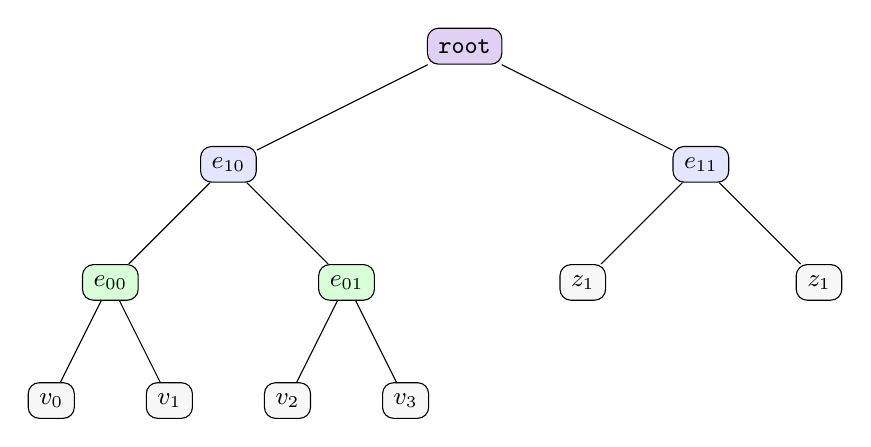
\begin{tikzpicture}[
  level 1/.style={sibling distance=6cm, level distance=1.5cm},
  level 2/.style={sibling distance=3cm, level distance=1.5cm},
  level 3/.style={sibling distance=1.5cm, level distance=1.5cm},
  every node/.style={draw, rounded corners, fill=backcolour,
                     font=\small\ttfamily, inner sep=4pt}
]
\node[fill=aztecpurple!20] {root}
  child { node[fill=blue!10] {$e_{10}$}
    child { node[fill=green!15] {$e_{00}$}
      child { node {$v_0$} }
      child { node {$v_1$} }
    }
    child { node[fill=green!15] {$e_{01}$}
      child { node {$v_2$} }
      child { node {$v_3$} }
    }
  }
  child { node[fill=blue!10] {$e_{11}$}
    child { node {$z_1$} }
    child { node {$z_1$} }
  };
\end{tikzpicture}

\medskip
\small $e_{00} = H(H(v_0)\|H(v_1))$, \quad $e_{01} = H(H(v_2)\|H(v_3))$, \quad
$e_{10} = H(e_{00}\|e_{01})$, \quad $e_{11} = H(z_1\|z_1) = z_2$
\end{center}

% =============================================================================
\section{Algorithm Design}
% =============================================================================

\subsection{Zero-Hash Pre-computation}

Both implementations pre-compute all $d+1$ zero hashes in the constructor
($O(d)$ hash calls).  These are stored in a length-$(d+1)$ array and used
wherever a node is absent from the database.

\subsection{\texttt{updateElement} — Leaf Update}

\begin{tcolorbox}[title=Algorithm: updateElement(index, value)]
\begin{enumerate}[label=\textbf{Step \arabic*:}]
  \item Compute $c \leftarrow H(\texttt{value})$  (leaf hash).
  \item Set $p \leftarrow \texttt{index}$, prepare an empty batch.
  \item \textbf{For} $k = 0$ \textbf{to} $d-1$:
    \begin{enumerate}[label=(\alph*)]
      \item Add $(k, p) \mapsto c$ to the write batch.
      \item $s \leftarrow p \oplus 1$  (sibling position).
      \item $\sigma \leftarrow \mathrm{getNode}(k, s)$
            (from DB or $z_k$ if absent).
      \item If $p$ is even: $c \leftarrow H(c \| \sigma)$,
            else $c \leftarrow H(\sigma \| c)$.
      \item $p \leftarrow p \gg 1$.
    \end{enumerate}
  \item $\texttt{root} \leftarrow c$.
  \item Commit the batch (including updated metadata).
  \item Return \texttt{root}.
\end{enumerate}
\end{tcolorbox}

\textbf{Complexity.} Each call performs exactly $d$ hash compressions and $d$
database reads (sibling lookups) plus $d+1$ database writes (path nodes +
metadata) — all $O(d)$ with $d = 32$.

\subsection{\texttt{getHashPath} — Membership Proof}

\begin{tcolorbox}[title=Algorithm: getHashPath(index)]
\begin{enumerate}[label=\textbf{Step \arabic*:}]
  \item Initialise an empty list \texttt{pairs}.
  \item \textbf{For} $k = 0$ \textbf{to} $d-1$:
    \begin{enumerate}[label=(\alph*)]
      \item $p \leftarrow \texttt{index} \gg k$.
      \item $p_L \leftarrow p \mathbin{\&} \mathord{\sim}1$,\quad
            $p_R \leftarrow p \mathbin{|} 1$.
      \item $L \leftarrow \mathrm{getNode}(k, p_L)$,\quad
            $R \leftarrow \mathrm{getNode}(k, p_R)$.
      \item Append $(L, R)$ to \texttt{pairs}.
    \end{enumerate}
  \item Return \texttt{HashPath(pairs)}.
\end{enumerate}
\end{tcolorbox}

Note that both indices $0$ and $1$ share the \emph{same} pair at level 0
(namely $(H(v_0), H(v_1))$), which is why the test asserts
\texttt{getHashPath(0) == getHashPath(1)} for a 2-leaf group.

\subsection{Database Persistence}

\begin{center}
\begin{tabular}{lll}
\toprule
\textbf{Key} & \textbf{Value} & \textbf{Purpose} \\
\midrule
\texttt{name} & 40 bytes: root (32) + depth (4, LE) & Tree metadata \\
\texttt{name:k:p} & 32 bytes: SHA-256 hash & Node at level $k$, position $p$ \\
\bottomrule
\end{tabular}
\end{center}

On construction, if no metadata entry exists the empty root $z_d$ is stored.
When \texttt{updateElement} finishes, the metadata key is atomically updated
alongside the path nodes using a batched write.

% =============================================================================
\section{TypeScript Implementation}
% =============================================================================

The TypeScript implementation is in
\texttt{eng-sessions/merkle-tree/src/merkle\_tree.ts}.

\subsection{Constructor}

\begin{lstlisting}[style=tscode, caption={TypeScript constructor — zero hash computation and root initialisation}]
constructor(private db: LevelUp, private name: string,
            private depth: number, root?: Buffer) {
  if (!(depth >= 1 && depth <= MAX_DEPTH)) throw Error('Bad depth');

  // Pre-compute z_0 ... z_depth
  this.zeroHashes = this.computeZeroHashes(depth);

  if (root) {
    this.root = root;           // restore from DB
  } else {
    this.root = this.zeroHashes[depth];  // fresh empty tree
  }
}

private computeZeroHashes(depth: number): Buffer[] {
  const zeros: Buffer[] = new Array(depth + 1);
  zeros[0] = this.hasher.hash(Buffer.alloc(LEAF_BYTES)); // H(0^64)
  for (let i = 1; i <= depth; i++) {
    zeros[i] = this.hasher.compress(zeros[i-1], zeros[i-1]);
  }
  return zeros;
}
\end{lstlisting}

\subsection{updateElement}

\begin{lstlisting}[style=tscode, caption={TypeScript updateElement — path traversal with batched writes}]
async updateElement(index: number, value: Buffer) {
  const batch = this.db.batch();
  let currentHash = this.hasher.hash(value);
  let pos = index;

  for (let level = 0; level < this.depth; level++) {
    batch.put(this.nodeKey(level, pos), currentHash);

    const siblingPos = pos ^ 1;
    const sibling = await this.getNode(level, siblingPos);

    if (pos % 2 === 0) {
      currentHash = this.hasher.compress(currentHash, sibling);
    } else {
      currentHash = this.hasher.compress(sibling, currentHash);
    }
    pos = pos >> 1;
  }

  this.root = currentHash;
  this.writeMetaData(batch);
  await batch.write();
  return this.root;
}
\end{lstlisting}

\subsection{getHashPath}

\begin{lstlisting}[style=tscode, caption={TypeScript getHashPath — returning sibling pairs}]
async getHashPath(index: number) {
  const pairs: Buffer[][] = [];

  for (let level = 0; level < this.depth; level++) {
    const pos   = index >> level;
    const leftPos  = pos & ~1;
    const rightPos = pos | 1;

    const left  = await this.getNode(level, leftPos);
    const right = await this.getNode(level, rightPos);

    pairs.push([left, right]);
  }

  return new HashPath(pairs);
}
\end{lstlisting}

\subsection{Test Results}

\begin{center}
\begin{tabular}{clcc}
\toprule
\textbf{\#} & \textbf{Test description} & \textbf{Expected root (hex prefix)} & \textbf{Pass?} \\
\midrule
1 & Empty depth-32 tree root & \texttt{1c9a7e5f\ldots} & \checkmark \\
2 & Depth-2 tree, 4 leaves, root + hash paths & \texttt{e645e6b5\ldots} & \checkmark \\
3 & Depth-10, 128 inserts, restore from DB & \texttt{4b8404d0\ldots} & \checkmark \\
4 & Depth-32, 1024 inserts, root + path[100] & \texttt{26996bfc\ldots} & \checkmark \\
\bottomrule
\end{tabular}
\end{center}

% =============================================================================
\section{C++20 Implementation}
% =============================================================================

The C++ implementation is in
\texttt{eng-sessions/merkle-tree-cpp/src/merkle\_tree.hpp}.

\subsection{Constructor}

\begin{lstlisting}[style=cppcode, caption={C++ constructor — zero hash pre-computation and DB restoration}]
MerkleTree(MockDB& db, const std::string& name,
           uint32_t depth, const sha256_hash_t& root = {})
    : db(db), name(name), depth(depth), root(root), hasher()
{
    if (!(depth >= 1 && depth <= MAX_DEPTH))
        throw std::runtime_error("Bad depth");

    // Pre-compute z_0 ... z_depth
    zero_hashes.resize(depth + 1);
    zero_hashes[0] = hasher.hash(std::vector<uint8_t>(LEAF_BYTES, 0));
    for (uint32_t i = 1; i <= depth; ++i)
        zero_hashes[i] = hasher.compress(zero_hashes[i-1], zero_hashes[i-1]);

    // Restore root from DB if present
    auto stored = db.get(name);
    if (stored.has_value()) {
        this->root = stored.value();
    } else {
        this->root = zero_hashes[depth];
        db.put(name, this->root);
    }
}
\end{lstlisting}

\subsection{update\_element}

\begin{lstlisting}[style=cppcode, caption={C++ update\_element — path traversal with batch write}]
sha256_hash_t update_element(uint64_t index,
                              const std::vector<uint8_t>& value)
{
    if (value.size() != LEAF_BYTES)
        throw std::runtime_error("Value must be exactly 64 bytes.");

    std::vector<MockDBBatchItem> batch;
    sha256_hash_t current_hash = hasher.hash(value);
    uint64_t pos = index;

    for (uint32_t level = 0; level < depth; ++level) {
        batch.push_back({ node_key(level, pos), current_hash });

        uint64_t sibling_pos = pos ^ uint64_t(1);
        sha256_hash_t sibling = get_node(level, sibling_pos);

        if (pos % 2 == 0)
            current_hash = hasher.compress(current_hash, sibling);
        else
            current_hash = hasher.compress(sibling, current_hash);

        pos >>= 1;
    }

    root = current_hash;
    batch.push_back({ name, root });
    db.batch_write(batch);
    return root;
}
\end{lstlisting}

\subsection{get\_hash\_path}

\begin{lstlisting}[style=cppcode, caption={C++ get\_hash\_path — returning sibling pairs as HashPath}]
HashPath get_hash_path(uint64_t index) const
{
    std::vector<std::pair<sha256_hash_t, sha256_hash_t>> pairs;
    pairs.reserve(depth);

    for (uint32_t level = 0; level < depth; ++level) {
        uint64_t pos       = index >> level;
        uint64_t left_pos  = pos & ~uint64_t(1);
        uint64_t right_pos = pos | uint64_t(1);

        sha256_hash_t left  = get_node(level, left_pos);
        sha256_hash_t right = get_node(level, right_pos);

        pairs.push_back({ left, right });
    }

    return HashPath(pairs);
}
\end{lstlisting}

\subsection{Test Results}

\begin{center}
\begin{tabular}{clcc}
\toprule
\textbf{\#} & \textbf{Test description} & \textbf{Expected root (hex prefix)} & \textbf{Pass?} \\
\midrule
1 & Empty depth-32 tree root & \texttt{1c9a7e5f\ldots} & \checkmark \\
2 & Depth-2 tree, 4 leaves, root + hash paths & \texttt{e645e6b5\ldots} & \checkmark \\
3 & Depth-10, 128 inserts, restore from DB & \texttt{4b8404d0\ldots} & \checkmark \\
4 & Depth-32, 1024 inserts, root + path[100] & \texttt{26996bfc\ldots} & \checkmark \\
\bottomrule
\end{tabular}
\end{center}

% =============================================================================
\section{Worked Example: Depth-2, 4 Leaves}
% =============================================================================

Let $v_i$ be a 64-byte value with $i$ encoded in the first 4 bytes
(little-endian), all other bytes zero.  Define:
\[
  e_{00} = H(v_0), \quad e_{01} = H(v_1), \quad e_{02} = H(v_2), \quad e_{03} = H(v_3).
\]
\[
  e_{10} = H(e_{00} \| e_{01}), \quad e_{11} = H(e_{02} \| e_{03}).
\]
\[
  \text{root} = H(e_{10} \| e_{11}).
\]

The test asserts:
\[
  \text{root} = \texttt{e645e6b5445483a358c4d15c1923c616a0e6884906b05c196d341ece93b2de42}.
\]

Hash paths:
\begin{align*}
  \Pi_0 = \Pi_1 &= \bigl((e_{00},\, e_{01}),\; (e_{10},\, e_{11})\bigr), \\
  \Pi_2 = \Pi_3 &= \bigl((e_{02},\, e_{03}),\; (e_{10},\, e_{11})\bigr).
\end{align*}

\textbf{Verification of $\Pi_0$:}
\begin{enumerate}
  \item $c = H(v_0) = e_{00}$.
  \item Level 0 pair $(e_{00}, e_{01})$: $c = H(e_{00} \| e_{01}) = e_{10}$.
  \item Level 1 pair $(e_{10}, e_{11})$: $c = H(e_{10} \| e_{11}) = \text{root}$.  \checkmark
\end{enumerate}

% =============================================================================
\section{Topics Covered — What This Problem Tests}
% =============================================================================

\subsection{Core Data Structures \& Algorithms}

\begin{itemize}
  \item \textbf{Binary trees and tree traversal}: The leaf-to-root path
        traversal is a fundamental tree operation used in databases
        (B-trees, red-black trees) and cryptographic protocols.

  \item \textbf{Sparse data structures}: Using zero-hash placeholders instead
        of materialising $2^{32}$ nodes — a common pattern in
        \emph{sparse Merkle trees} used in Ethereum, Solana, and zkRollups.

  \item \textbf{Hashing as a commitment scheme}: SHA-256 as a one-way,
        collision-resistant function used to bind data.

  \item \textbf{Bit manipulation}: Sibling address via XOR ($p \oplus 1$),
        left/right detection via even/odd ($p \bmod 2$), level shift via
        $p \gg k$.
\end{itemize}

\subsection{Cryptography Topics}

\begin{itemize}
  \item \textbf{Hash functions}: SHA-256 — construction, collision resistance,
        preimage resistance, the avalanche effect.

  \item \textbf{Merkle trees in practice}: Blockchain state roots
        (Bitcoin transactions, Ethereum MPT), certificate transparency logs,
        content-addressable storage (IPFS, Git).

  \item \textbf{Merkle proofs}: Succinct membership proofs, $O(\log N)$
        verification; used inside zkSNARKs (Groth16, PLONK, Honk) to prove
        knowledge of a private leaf in a public tree.

  \item \textbf{Commitment schemes}: A Merkle root commits to all leaves;
        updating a leaf is an $O(d)$ re-commitment operation.
\end{itemize}

\subsection{Systems / Engineering Topics}

\begin{itemize}
  \item \textbf{Key--value persistence}: LevelUp (TypeScript) /
        \texttt{unordered\_map} (C++); designing a key schema that uniquely
        identifies each tree node.

  \item \textbf{Batched writes}: Grouping all path-node writes plus the
        metadata update into a single atomic batch — important for
        crash-consistency and performance.

  \item \textbf{Database restoration}: Serialising / deserialising tree state
        (root + depth) to reconstruct a live tree object from a cold store.

  \item \textbf{Async/await patterns} (TypeScript): LevelUp operations are
        Promise-based; the implementation carefully awaits each DB read while
        batching all writes.

  \item \textbf{Generic programming} (C++20): Template utilities
        (\texttt{to\_hex}, \texttt{assert\_equal\_hex}),
        \texttt{std::optional}, \texttt{std::array}, \texttt{std::vector}.
\end{itemize}

\subsection{Aztec-Specific Context}

Aztec Protocol uses Merkle trees extensively:
\begin{itemize}
  \item \textbf{Note commitment tree}: A sparse Merkle tree that stores UTXO
        note commitments; the root is part of every Aztec block header.
  \item \textbf{Nullifier tree}: An indexed Merkle tree used to prevent
        double-spending without revealing which note was spent.
  \item \textbf{Archive tree}: Stores a history of all past block headers,
        enabling proofs about historical state.
  \item \textbf{SNARK circuits}: The \texttt{getHashPath} result is passed
        as a witness into Noir/Barretenberg circuits, which re-verify the
        membership proof in zero-knowledge.
\end{itemize}

% =============================================================================
\section{Complexity Summary}
% =============================================================================

\begin{center}
\begin{tabular}{lll}
\toprule
\textbf{Operation} & \textbf{Time} & \textbf{Space} \\
\midrule
Constructor (zero hashes) & $O(d)$ hash ops & $O(d)$ \\
\texttt{updateElement} & $O(d)$ hash ops + $O(d)$ DB I/O & $O(d)$ \\
\texttt{getHashPath} & $O(d)$ DB reads & $O(d)$ \\
\texttt{getRoot} & $O(1)$ & $O(1)$ \\
\midrule
Total storage per tree & $O(N \cdot d)$ & where $N$ = \# of updates \\
\bottomrule
\end{tabular}
\end{center}

With $d = 32$, each \texttt{updateElement} call touches at most 32 nodes per
path, so inserting $N$ leaves costs $O(N \cdot d)$ hash operations overall.

% =============================================================================
\section{Conclusion}
% =============================================================================

Both the TypeScript and C++ Merkle tree implementations pass all four test
cases.  The key design choices are:
\begin{enumerate}
  \item Pre-compute zero hashes in the constructor to handle sparse nodes
        without storing them.
  \item Use string keys \texttt{name:level:pos} in the database for O(1)
        node lookup.
  \item Traverse from leaf to root in a single loop for both
        \texttt{updateElement} (writing) and \texttt{getHashPath} (reading).
  \item Persist all writes atomically via a database batch, including the
        metadata root update.
\end{enumerate}

\vspace{1cm}
\begin{center}
  {\color{aztecpurple}\rule{0.5\linewidth}{1pt}}\\[0.3cm]
  \textit{Solution implemented and all 8 tests passing (4 TypeScript + 4 C++).}\\[0.3cm]
  {\color{aztecpurple}\rule{0.5\linewidth}{1pt}}
\end{center}

\end{document}
